%%%%%%%% DA-3041 Group 9 supplementary material %%%%%%%%%%%%%%%%%

\documentclass{article}

\usepackage{microtype}
\usepackage{graphicx}
\usepackage{booktabs}
\usepackage{amsmath}
\usepackage{amssymb}
\usepackage{algorithm}
\usepackage{algorithmic}
\usepackage{hyperref}

\usepackage[accepted]{icml2018}

% course report, not an ICML publication: replace the "appearing in" footnote
\makeatletter
\renewcommand{\ICML@appearing}{DA-3041 Applied Time Series Analysis course project, IIT Guwahati, 2026.}
\makeatother

\icmltitlerunning{Supplementary Material: Wavelet + ARMA--GARCH Volatility Forecasting}

\begin{document}

\twocolumn[
\icmltitle{Supplementary Material for\\
``Does Splitting Returns with Wavelets Help GARCH Forecast Volatility?''}

\begin{icmlauthorlist}
\icmlauthor{Neeharika}{iitg}
\icmlauthor{Pratyaksha Jha}{iitg}
\icmlauthor{Pushpendra Singh}{iitg}
\icmlauthor{Somita Agarwal}{iitg}
\end{icmlauthorlist}

\icmlaffiliation{iitg}{Indian Institute of Technology Guwahati, India. DA-3041 Applied Time Series Analysis, Group 9}

\icmlcorrespondingauthor{Pushpendra Singh}{github.com/pushpendras0026}

\vskip 0.3in
]

\printAffiliationsAndNotice{}

\section{Code}

All code, data, configuration, tests and result tables are here:

\begin{center}
\url{https://github.com/pushpendras0026/Volatility-forecasting-with-the-wavelet-transform}
\end{center}

The repository README explains how to run everything with one command (\texttt{Rscript run\_all.R --workers 16}). It needs only R 4.6 with the recommended package \texttt{nnet}, no internet. The run first does the unit and leakage tests, then all forecasts, then the tables and figures, then the innovation-distribution experiment. The recorded model-fitting time of the final run is about 3.8 CPU-hours in total, spread over the workers. The bulky raw forecast files are stored as zip files in the repository and only need to be unzipped if you want to re-make the tables without re-running the models.

\section{How to implement the method}

This section describes the full procedure in words and pseudocode, so somebody can re-build it without our code.

\subsection{Data preparation}
\begin{enumerate}
\item Read daily closing prices, sort by date, drop duplicate dates. Do not fill missing days.
\item Compute $r_t=\ln P_t-\ln P_{t-1}$ (decimal, not percent).
\item Compute the target $y_{t+1}=(r_{t+1}-\bar r^{(20)}_t)^2$ where $\bar r^{(20)}_t$ is the mean of $r_{t-19},\dots,r_t$.
\item Split by calendar: training up to 31 Dec 2009, validation 2010--2011, test 2012--2014, later period 2015--2025 (stocks only).
\end{enumerate}

\subsection{Rolling forecast loop}

\begin{algorithm}[h]
\caption{Rolling one-step forecast for one model}
\begin{algorithmic}
\STATE {\bfseries Input:} returns $r_{1..T}$, first forecast origin $t_0$, window $W=1024$, refit cadence $K=20$, frozen order $(p,q)$
\FOR{$t=t_0$ {\bfseries to} $T-1$}
\IF{$(t-t_0)$ mod $K = 0$ or last fit failed}
\STATE take the last $W$ observations up to $t$
\STATE transform them (raw / paired DWT / MODWT)
\STATE fit ARMA$(p,q)$ by Gaussian ML
\STATE fit GARCH(1,1) on its residuals by ML
\ELSE
\STATE keep parameters, update ARMA state and $h_t$ with the new observation
\ENDIF
\STATE get one-step $\mu$ and $h$ of the input series
\STATE map them to return moments $\mu_{t+1},h_{t+1}$
\STATE $\hat y_{t+1}=h_{t+1}+(\mu_{t+1}-\bar r^{(20)}_t)^2$
\ENDFOR
\end{algorithmic}
\end{algorithm}

A failed fit is tried again at the next day; we never fall back silently to an old fit, and the failed day is marked missing. Comparisons then use only dates where all compared models have a forecast.

\subsection{Order selection}
On the last 1,024 training observations, fit every ARMA$(p,q)$ with $0\le p,q\le3$ and keep the one with the lowest AIC $=-2\ell+2k$, where $k$ counts the ARMA coefficients, the constant and the variance. This order is then frozen for validation and test. For the paired DWT, the order is chosen separately for the approximation and the detail series. Table~\ref{tab:orders} lists the chosen orders and the GARCH parameters of the first fit.

\begin{table}[t]
\caption{ARMA orders chosen by AIC and the first GARCH(1,1) fit at the end of training (Gaussian). DWT has two series: detail ($d$) and approximation ($a$).}
\label{tab:orders}
\centering\small
\setlength{\tabcolsep}{3pt}
\begin{tabular}{llcrr}
\toprule
Series & Model & $(p,q)$ & $\alpha$ & $\beta$\\
\midrule
S.\ Africa & raw & (3,1) & 0.113 & 0.873\\
 & DWT $d$ / $a$ & (2,2) / (3,3) & 0.189 / 0.116 & 0.784 / 0.855\\
 & MODWT & (3,2) & 0.116 & 0.868\\
Tunisia & raw & (2,0) & 0.166 & 0.760\\
 & DWT $d$ / $a$ & (2,3) / (1,2) & 0.244 / 0.184 & 0.631 / 0.619\\
 & MODWT & (2,1) & 0.164 & 0.761\\
Nigeria & raw & (0,3) & 0.155 & 0.790\\
 & DWT $d$ / $a$ & (3,0) / (0,1) & 0.207 / 0.118 & 0.566 / 0.881\\
 & MODWT & (3,1) & 0.152 & 0.791\\
Infosys & raw & (0,3) & 0.108 & 0.872\\
 & DWT $d$ / $a$ & (3,2) / (2,2) & 0.169 / 0.063 & 0.773 / 0.926\\
 & MODWT & (2,2) & 0.115 & 0.865\\
IBM & raw & (2,2) & 0.079 & 0.904\\
 & DWT $d$ / $a$ & (3,3) / (2,2) & 0.096 / 0.082 & 0.881 / 0.894\\
 & MODWT & (2,3) & 0.077 & 0.906\\
Google & raw & (3,2) & 0.049 & 0.948\\
 & DWT $d$ / $a$ & (2,2) / (1,1) & 0.073 / 0.062 & 0.922 / 0.920\\
 & MODWT & (0,1) & 0.050 & 0.947\\
\bottomrule
\end{tabular}
\end{table}

\subsection{GARCH likelihoods}
Given ARMA residuals $\varepsilon_t$, the variance follows $h_t=\omega+\alpha\varepsilon_{t-1}^2+\beta h_{t-1}$, started at the sample variance. We maximise the log-likelihood with box constraints $\omega>0$, $\alpha,\beta\ge0$, $\alpha+\beta<1$:
\begin{itemize}
\item Gaussian: $\ell=-\tfrac12\sum[\ln(2\pi h_t)+\varepsilon_t^2/h_t]$.
\item Student-t with $\nu>2$, scaled to unit variance: $z_t=\varepsilon_t/\sqrt{h_t}$ has density $\frac{\Gamma(\frac{\nu+1}{2})}{\Gamma(\frac\nu2)\sqrt{\pi(\nu-2)}}\bigl(1+\frac{z^2}{\nu-2}\bigr)^{-\frac{\nu+1}{2}}$, minus $\tfrac12\ln h_t$.
\item GED with shape $\kappa$, unit variance: density $\frac{\kappa\exp(-\frac12|z/\lambda|^\kappa)}{\lambda\,2^{1+1/\kappa}\Gamma(1/\kappa)}$ with $\lambda=\bigl(2^{-2/\kappa}\Gamma(1/\kappa)/\Gamma(3/\kappa)\bigr)^{1/2}$. $\kappa=2$ is Gaussian and $\kappa<2$ has fatter tails.
\end{itemize}

\subsection{Wavelet transforms}
\textbf{Haar MODWT, level 1.} $w_t=(r_t-r_{t-1})/2$, one value per day. Given $(\mu_w,h_w)$ for $w_{t+1}$, $\mu_r=r_t+2\mu_w$, $h_r=4h_w$.

\textbf{Paired Haar DWT.} Make pairs from the newest complete pair backwards, $(u_k,v_k)=(r_{t-2j-1},r_{t-2j})$ ending with $(r_{t-2},r_{t-1})$ (an odd leftover at the oldest end is dropped). Compute $a_k=(u_k+v_k)/\sqrt2$ and $d_k=(v_k-u_k)/\sqrt2$, fit one ARMA--GARCH to each, and combine with the conditional formulas in Section 3.3 of the main report, where $s=\sqrt2\,r_t$ is the known part of the next pair.

\textbf{Component models (E3).} At each origin, decompose the observed history of $y$ (DWT or MODWT, Haar/db4/db6, $J=1,2$) with reflection at the edges, so only past data is used. Forecast each of $A_J,D_J,\dots,D_1$ one step ahead and add the forecasts; clip the final sum at zero. Figure~\ref{fig:comp} shows a Haar MODWT split with $J=2$.

\begin{figure}[t]
\centering
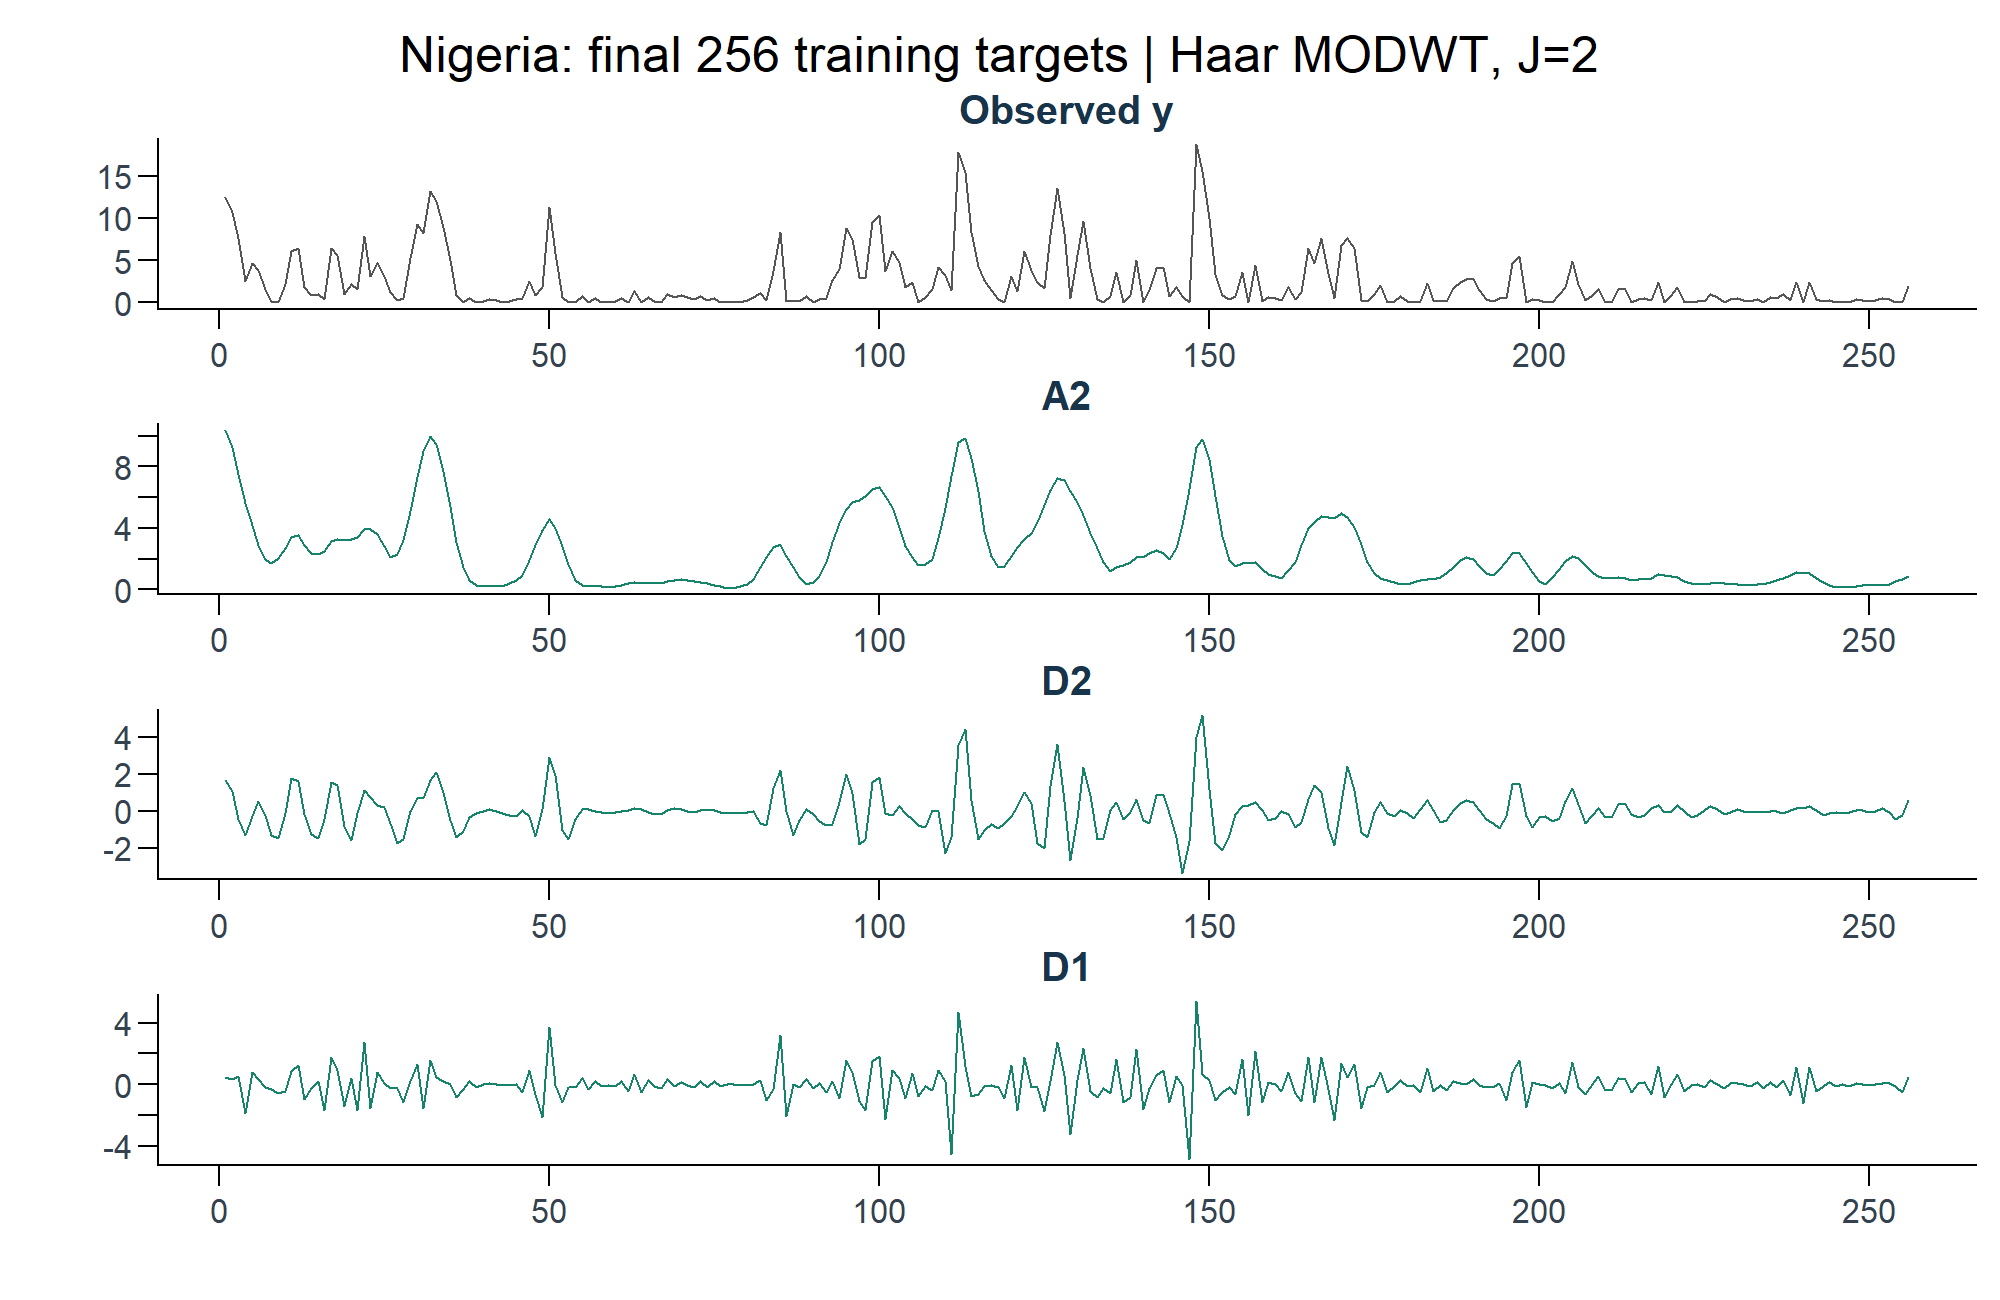
\includegraphics[width=\columnwidth]{figures/component_example.png}
\caption{Nigeria, last 256 training targets ($\times10^4$) and their Haar MODWT parts with $J=2$. The parts add up to the observed series.}
\label{fig:comp}
\end{figure}

\subsection{Ensembles and MLP}
Ensemble forecasts are the plain average of the member forecasts on the same day. If any member is missing that day, the ensemble is missing too (we do not average fewer members). The MLP uses inputs $(y_t,\dots,y_{t-4},\bar y^{(5)}_t,\bar y^{(20)}_t)$, standardised with training means and standard deviations, one hidden sigmoid layer, a linear output, at most 300 iterations; fits that hit the iteration limit are marked as unavailable.

\section{Extra results}

\begin{table}[t]
\caption{Sensitivity: MSE gain (\%) of each setting change vs.\ the default (window 1024, refit 20, AIC, cap 3), raw GARCH, test 2012--2014. Pairwise matched dates.}
\label{tab:sens}
\centering\small
\setlength{\tabcolsep}{2.5pt}
\begin{tabular}{lrrrrrr}
\toprule
Change & SA & Tun & Nig & Inf & IBM & Goog\\
\midrule
Window 768 & 1.15 & $-14.36$ & 1.77 & $-0.19$ & 0.36 & 0.08\\
Window 1536 & $-0.26$ & 7.93 & 7.19 & 0.36 & $-1.98$ & $-1.61$\\
Refit 40 & 0.40 & 0.02 & $-1.55$ & $-0.07$ & $-0.27$ & 0.06\\
Refit 60 & 0.37 & 2.31 & $-1.76$ & $-0.64$ & $-0.75$ & 0.01\\
BIC & $-0.10$ & 0.34 & 0.00 & 1.23 & 0.07 & 0.26\\
Order cap 5 & $-0.32$ & $-2.56$ & 0.07 & $-0.32$ & $-1.02$ & 0.10\\
\bottomrule
\end{tabular}
\end{table}

\begin{table}[t]
\caption{Test RMSE $\times10^4$ (2012--2014) for DWT and MODWT pipelines under the three innovation distributions. Dates where all three distributions have a forecast.}
\label{tab:dist2}
\centering\small
\setlength{\tabcolsep}{3pt}
\begin{tabular}{llrrr}
\toprule
Series & Pipeline & Gaussian & Student-t & GED\\
\midrule
S.\ Africa & DWT & 1.3448 & 1.3448 & 1.3448\\
 & MODWT & 1.3394 & 1.3389 & 1.3391\\
Tunisia & DWT & 0.6790 & 0.6564 & 0.6622\\
 & MODWT & 0.7061 & 0.7013 & 0.7023\\
Nigeria & DWT & 1.8015 & 1.8090 & 1.8042\\
 & MODWT & 1.9173 & 1.9073 & 1.9129\\
Infosys & DWT & 24.9339 & 24.8529 & 24.9561\\
 & MODWT & 25.1997 & 25.0508 & 25.1189\\
IBM & DWT & 4.1669 & 4.1766 & 4.1679\\
 & MODWT & 4.1395 & 4.1400 & 4.1367\\
Google & DWT & 7.7759 & 7.7907 & 7.7822\\
 & MODWT & 7.7684 & 7.7564 & 7.7489\\
\bottomrule
\end{tabular}
\end{table}

\begin{table}[t]
\caption{MLP seeds vs.\ raw GARCH, test RMSE $\times10^4$, on dates where raw GARCH, all three MLP seeds and the three ensembles have a forecast.}
\label{tab:mlp}
\centering\small
\setlength{\tabcolsep}{3pt}
\begin{tabular}{lrrrrr}
\toprule
Series & $n$ & Raw & Seed 101 & Seed 202 & Seed 303\\
\midrule
S.\ Africa & 688 & 1.3771 & 1.5194 & 1.5140 & 1.4648\\
Tunisia & 540 & 0.3794 & 0.4083 & 0.4201 & 0.5413\\
Nigeria & 745 & 1.8920 & 2.4044 & 2.0768 & 2.0256\\
Infosys & 199 & 23.1670 & 33.2734 & 24.0858 & 33.2707\\
IBM & 751 & 4.1300 & 4.2190 & 4.1655 & 4.2011\\
Google & 704 & 7.9898 & 8.1453 & 8.0270 & 8.0803\\
\bottomrule
\end{tabular}
\end{table}

Tables~\ref{tab:sens}--\ref{tab:mlp} give more detail on the results in the main report. In Table~\ref{tab:mlp} the number of dates is small for Infosys (199) because some MLP and ensemble forecasts were missing on many days; raw GARCH RMSE on these dates is different from the main table only because the dates are different.

\textbf{Matched-date rule.} Every number in our result files comes with a \texttt{sample\_rule} column that says which dates were used. The file \texttt{tables/sample\_reconciliation.csv} in the repository shows the same model under every rule, so the small differences between tables can be checked.

\end{document}
